\documentclass{beamer}
\usepackage[pantone315]{wwustyle}
\usepackage[ngerman]{babel}
\usepackage[utf8]{inputenc}
\usepackage{lmodern}

% \usepackage[style=verbose, backend=biber]{biblatex}
%\addbibresource{res/literatur.bib}
%\setbeamertemplate{bibliography item}{\insertbiblabel}

\usepackage{graphicx}
\graphicspath{{res/}{img/}{../img/}}
\usepackage{amsmath}
\usepackage{amssymb}
\usepackage{siunitx}

% Section-Ueberschrift Slides
\AtBeginSection[]{
  \begin{frame}
  \vfill
  \centering
  \begin{beamercolorbox}[sep=8pt,center,shadow=true,rounded=true]{title}
    \usebeamerfont{title}\insertsectionhead\par%
  \end{beamercolorbox}
  \vfill
  \end{frame}
}


\title[short title]{Title} %TODO add title
\subtitle{Subtitle} %TODO add subtitle
\institutelogo{}
\institutelogosmall{}
\author{Autor 1, Autor 2, Autor 3} %TODO add author
\date{01.01.1970} %TODO add date

\begin{document}

% Title
\begin{frame}[plain]
\maketitle
\end{frame}



\begin{frame}
\frametitle{Übersicht}

% Inhaltsverzeichnis
\tableofcontents

\end{frame}


\section{Motivation}

\begin{frame}
\frametitle{Motivation}
\begin{center}
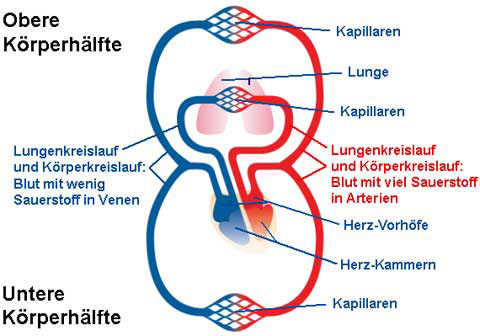
\includegraphics[scale=0.55]{motivation.jpg}  
\end{center}
\end{frame}

\section{Herleitung des 1D-Modells}




\begin{frame}\frametitle{Reynolds Transport Theorem}

  \begin{align}
    \frac{d}{dt} \int_{V_t} f dV = \int_{V_t} \frac{\partial f}{\partial t}dV + \int_{\partial V_t} f \vec u_w \cdot \vec n d\sigma \label{10.1} % 10.1
  \end{align}

  \begin{center}
      \includegraphics[width=0.5\textwidth]{vessel}
  \end{center}

\end{frame}


\begin{frame}\frametitle{Mittelung über Querschnitt}


  \begin{align}
    \bar f = \frac{1}{A} \int_S f d\sigma % 10.3
  \end{align}
  Damit lhs:
  \begin{align}
    \frac{d}{dt} \int_{V_t} f dV = \int_{x_1}^{x_2} \frac{\partial}{\partial t} (A \bar f) dx % 10.5
  \end{align}

\end{frame}


\begin{frame}\frametitle{Allgemeine 1D-Form}
  aus rhs mit Gauß-Theorem:
  \begin{equation}
  \begin{aligned}
    \int_{\partial V_{t,w}} f \vec u_w \cdot \vec n d\sigma = \int_{\partial V_{t, w}} f \vec w \cdot \vec n d\sigma &- \int_{x_1}^{x_2} \frac{\partial}{\partial x} \left[  A (\bar{f u_1}) \right] dx \\&+ \int_{V_t} \nabla \cdot (f \vec u) dV
  \end{aligned} % 10.6
\end{equation} %TODO: ist die Formel zu viel?
In Gl. (\ref{10.1}) \& x-Integration wegfallen lassen:
\begin{align}
\boxed{
\frac{\partial}{\partial t} (A \bar f) + \frac{\partial}{\partial x} \left[ A (\bar{f u_1}) \right] = \int_S \left[ \frac{\partial f}{\partial t}
+ \nabla \cdot (f\vec u) \right] d \sigma
+ \int_{\partial S} f \vec w \cdot \vec n d \gamma} % 10.7
\end{align}
\end{frame}

\begin{frame}\frametitle{Massenerhaltung}
Setze $f=1$ und $\nabla \cdot \vec u = 0$ (inkompressibel):
\begin{align}
  \frac{\partial A}{\partial t} + \frac{\partial}{\partial x} (A \bar u_1) = \int_{\partial S} \vec w \cdot \vec n d\gamma % 10.8
\end{align}
\end{frame}

\begin{frame}\frametitle{Impulserhaltung}
  Setze $f=u_1$, $\nabla \cdot \vec u = 0$, $\rho=$ const. und Annahme, dass Viskositätskraft linear in $\bar{u}$ ist:
\begin{align}
\boxed{
\frac{\partial}{\partial t} (A \bar u_1) + \frac{\partial}{\partial x} \left[ A \alpha \bar{u}_1^2 \right] = A \bar{f}^b_1 - \frac{A}{\rho}\left(\frac{\partial \vec{p}}{\partial x}\right)- K_R \bar{u}_1 + \int_{\partial S}u_1 \vec{w}\cdot \vec{n}\text{d}\sigma}
\end{align}
  mit der Materialableitung $\frac{D}{Dt}=\frac{\partial}{\partial t}+\vec{u}\cdot \nabla$, der Volumenkraft $\bar{f}^b_1$ und dem Korrekturfaktor $\bar{u^2}_1=\alpha \cdot \bar{u}_1^2$. %TODO sagen: alpha?1 z.b. flaches profil
  \end{frame}
%  \begin{frame}\frametitle{Herleitung}
%   Mit dem divergenz Theorem, der "constitutive" Gleichung, der Körperkraft pro Volumeneinheit $f^b$ und wieder weglassen von $x$-Integration:
%  \begin{align}
%  \int_S\frac{Du_1}{Dt}\text{d}\sigma = \int_S\left[f_1^b+\frac{1}{\rho}\left(-\frac{\partial p}{\partial x}+d_1\right)\right]
%  \end{align}
%  wobei $\nabla \cdot \vec{D}=\vec{d}$, mit $\vec{D}$ der deviatorische Stresstensor ist und $d_1$ die x-Komp. darstellt.
%\end{frame}
%\begin{frame}
%\frametitle{Herleitung}
%Da i.A. $\bar{u}_1^2\neq \bar{u^2}_1$, aber nur $\bar{u}_1^2$ bekannt, Korrekturterm:
%\begin{align}
%\bar{u^2}_1=\alpha \cdot \bar{u}_1^2
%\end{align}
%Die Viskousitätkraft $d_1$ ist lin. von $\bar{u}_1$ $\Rightarrow$
%\begin{align}
%\boxed{
%\frac{\partial}{\partial t} (A \bar u_1) + \frac{\partial}{\partial x} \left[ A \alpha \bar{u}_1^2 \right] = A \bar{f}^b_1 - \frac{A}{\rho}\left(\frac{\partial \vec{p}}{\partial x}\right)- K_R \bar{u}_1 + \int_{\partial S}u_1 \vec{w}\cdot \vec{n}\text{d}\sigma}
%\end{align}
%\end{frame}
\begin{frame}
\frametitle{Wall-Mechaniken}
Annahme: statisches Ggw. in radialen Richtung im Zylinder:
\begin{align}
p=P_\text{ext}+\beta(\sqrt{A}-\sqrt{A_0})
\end{align}
mit $\beta = \frac{\sqrt{\pi}h_0E}{(1-\nu^2)A_0}$.
\end{frame}



\begin{frame}
\frametitle{\textbf{Endformel}}
Mit der Annahme, dass die Innenwand undurchlässig ist ($\vec{w}\cdot \vec{n}=0$) und dass die Volumenkraft vernachlässigt werden können ($\bar{f}^b_1=0$), sowie $\alpha=1$ folgt:
\begin{align}
\boxed{\frac{\partial \vec{U}}{\partial t}+\frac{\partial \vec{F}}{\partial x}=\vec{S}(\vec{U})}
\end{align}
mit :
\begin{align*}
\vec{U}=\begin{pmatrix} A \\ u \end{pmatrix} \hspace{1cm} \vec{F}=\begin{pmatrix} Au \\ \frac{u^2}{2} + \frac{p}{\rho}
\end{pmatrix} \hspace{1cm} \vec{S}=\begin{pmatrix} 0 \\ -K_R \frac{u}{A}
\end{pmatrix}
\end{align*}
\end{frame}

\section{Das 0D-Modell}

\begin{frame}\frametitle{0D-Modell: Herleitung}

Weitere Mittelung:
\begin{align*}
  \hat p &= \frac{1}{l} \int_{x_1}^{x_2} P(x) dx~~~~~~~~
  \hat A = \frac{1}{l} \int_{x_1}^{x_2} A(x) dx\\
  \hat Q &= \frac{\rho}{l} \int_{x_1}^{x_2} Q(x) dx
\end{align*}
\pause
zusätzliche Annahmen:
\begin{itemize}
  \item vernachlässige Konvektion $\partial_x (\alpha Q^2 / A)$
  \item Querschnitt konstant: $A(x) = A_0$
  \item $\hat p \approx P_1$, $\hat Q \approx Q^2$
\end{itemize}

\end{frame}

%
% \begin{frame}\frametitle{0D-Modell: Herleitung}
% \begin{equation}
%   \begin{aligned}
%     C \frac{d\hat p}{dt} &= Q_1 - Q_2\\
%     L \frac{d\hat Q}{dt} &= P_1 - P_2 - RQ_2
%   \end{aligned}
% \end{equation}
%
% \end{frame}



\begin{frame}
\frametitle{0D-Modell: Analogie}
\begin{equation}
  \begin{aligned}
    C \frac{dP_1}{dt} &= Q_1 - Q_2\\
    L \frac{dQ_2}{dt} &= P_1 - P_2 - RQ_2
  \end{aligned}
\end{equation}
\pause
Analog zu elektrischen Bauteilen:
\begin{center}
  \includegraphics[width=0.6\textwidth]{kirchhoff.png}
\end{center}
\end{frame}

\begin{frame}
\frametitle{0D-Modell: Analogie}
  \begin{center}
  	\begin{tabular}[!htb]{c c c}
  		Hydraulisch	&	Variable	&	Elektrisch\\
  		\hline
  		Druck	&	$P$	&	Spannung\\
  		Flussrate	&	$Q$	&	Stromstärke\\
  		Blut-Viskosität	&	$R$	&	Widerstand\\
  		Blut-Trägheit	&	$L$	&	Induktivität\\
  		Ader-Elastizität	&	$C$	&	Kapazität
  	\end{tabular}
  \end{center}

\end{frame}


\begin{frame}
\frametitle{0D-Modell: Simulation}
\begin{columns}
  \begin{column}{0.45\textwidth}
    \begin{itemize}
      \item Numerische Lösung\\
      \item Python/\texttt{scipy}\\
      \item Runge-Kutta 4\\
      \item grobe Parameterwahl:\\
      {$P_{1/2}, Q_{1/2}, R, L, C = 1$}
    \end{itemize}
  \end{column}
  \begin{column}{0.55\textwidth}
    \begin{center}
      \centering
      \includegraphics[width=1.1\textwidth]{simulation1.pdf}\\
    \end{center}
  \end{column}
\end{columns}


\end{frame}

\section{Fazit}

\begin{frame}
\frametitle{Fazit}

\end{frame}


% Print bibliography
% \begin{frame}[t,allowframebreaks]
% \frametitle{Sources}
% 	\printbibliography
% \end{frame}

\end{document}
